\documentclass[aspectratio=169, 10pt]{beamer}

% --- Idioma e Codificação (Compatível universalmente) ---
\usepackage[utf8]{inputenc}
\usepackage[T1]{fontenc}
\usepackage{textcomp}

% Suporte a caracteres UTF-8 específicos
\DeclareUnicodeCharacter{00A7}{\S}
\DeclareUnicodeCharacter{00AA}{\textordfeminine}
\DeclareUnicodeCharacter{00BA}{\textordmasculine}

% --- Matemática e Símbolos ---
\usepackage{amsmath, amssymb, amsfonts, mathtools}
\usepackage{pifont} % Para \ding{51} e \ding{55}

% --- Elementos Visuais e Tipografia ---
\usepackage{graphicx}
\usepackage{booktabs}
\usepackage{array}
\usepackage{tikz}

% --- Configurações de Cores UNICAMP / Tema da Disciplina ---
\definecolor{unicampblue}{RGB}{24, 43, 73}
\definecolor{unicampteal}{RGB}{2, 132, 199}
\definecolor{accentgreen}{RGB}{16, 185, 129}
\definecolor{accentamber}{RGB}{217, 119, 6}
\definecolor{accentred}{RGB}{220, 38, 38}

% --- Configuração do Tema Beamer ---
\usetheme{default}
\usecolortheme{default}

\setbeamercolor{palette primary}{bg=unicampblue,fg=white}
\setbeamercolor{palette secondary}{bg=unicampteal,fg=white}
\setbeamercolor{palette tertiary}{bg=unicampblue!80,fg=white}
\setbeamercolor{structure}{fg=unicampblue}
\setbeamercolor{title}{fg=unicampblue}
\setbeamercolor{frametitle}{fg=unicampblue,bg=white}
\setbeamercolor{section title}{fg=white,bg=unicampblue}

% Blocos Nativos Estilizados
\setbeamertemplate{blocks}[rounded][shadow=false]
\setbeamercolor{block title}{bg=unicampblue, fg=white}
\setbeamercolor{block body}{bg=unicampblue!5!white, fg=black}

\setbeamercolor{block title example}{bg=accentgreen!80!black, fg=white}
\setbeamercolor{block body example}{bg=accentgreen!5!white, fg=black}

\setbeamercolor{block title alerted}{bg=accentred!90!black, fg=white}
\setbeamercolor{block body alerted}{bg=accentred!5!white, fg=black}

% Fontes e espaçamentos
\setbeamerfont{title}{size=\Large, series=\bfseries}
\setbeamerfont{subtitle}{size=\small, series=\mdseries}
\setbeamerfont{frametitle}{size=\large, series=\bfseries}
\setbeamertemplate{navigation symbols}{} % Remove os botões de navegação pequenos

% Rodapé elegante com número de slide
\setbeamertemplate{footline}{
  \leavevmode%
  \hbox{%
  \begin{beamercolorbox}[wd=.75\paperwidth,ht=2.5ex,dp=1ex,left,leftskip=1cm]{palette secondary}%
    \usebeamerfont{author in head/foot}\textbf{UNICAMP} --- Instituto de Computação \quad$\vert$\quad Álgebra Linear e Otimização para ML
  \end{beamercolorbox}%
  \begin{beamercolorbox}[wd=.25\paperwidth,ht=2.5ex,dp=1ex,right,rightskip=1cm]{palette secondary}%
    \insertframenumber{} / \inserttotalframenumber
  \end{beamercolorbox}}%
  \vskip0pt%
}

% --- Ambientes de Callout mapeados para Blocos Nativos do Beamer ---
\newenvironment{calloutnote}[1][Nota]{%
  \begin{block}{#1}%
}{%
  \end{block}%
}

\newenvironment{callouttip}[1][Dica]{%
  \begin{exampleblock}{#1}%
}{%
  \end{exampleblock}%
}

\newenvironment{calloutwarning}[1][Atenção]{%
  \begin{alertblock}{#1}%
}{%
  \end{alertblock}%
}

\newenvironment{calloutimportant}[1][Importante]{%
  \begin{alertblock}{#1}%
}{%
  \end{alertblock}%
}

% Comandos para V/F
\newcommand{\cmark}{\textcolor{green!60!black}{\textbf{\ding{51}}}}
\newcommand{\xmark}{\textcolor{red!70!black}{\textbf{\ding{55}}}}
\newcommand{\qmark}{\textbf{$\square$}}

% --- Metadados da Apresentação ---
\title{Aula 11: Otimização de Segunda Ordem (Método de Newton) e Precondicionamento Diagonal}
\subtitle{Otimização e Álgebra Linear para Machine Learning}
\author{Prof. Marcos M. Raimundo}
\institute{Instituto de Computação --- UNICAMP}
\date{Segundo Semestre de 2026}

\begin{document}

% ==============================================================================
% SLIDE 0: CAPA
% ==============================================================================
\begin{frame}[plain]
  \vspace{0.3cm}
  \begin{center}
    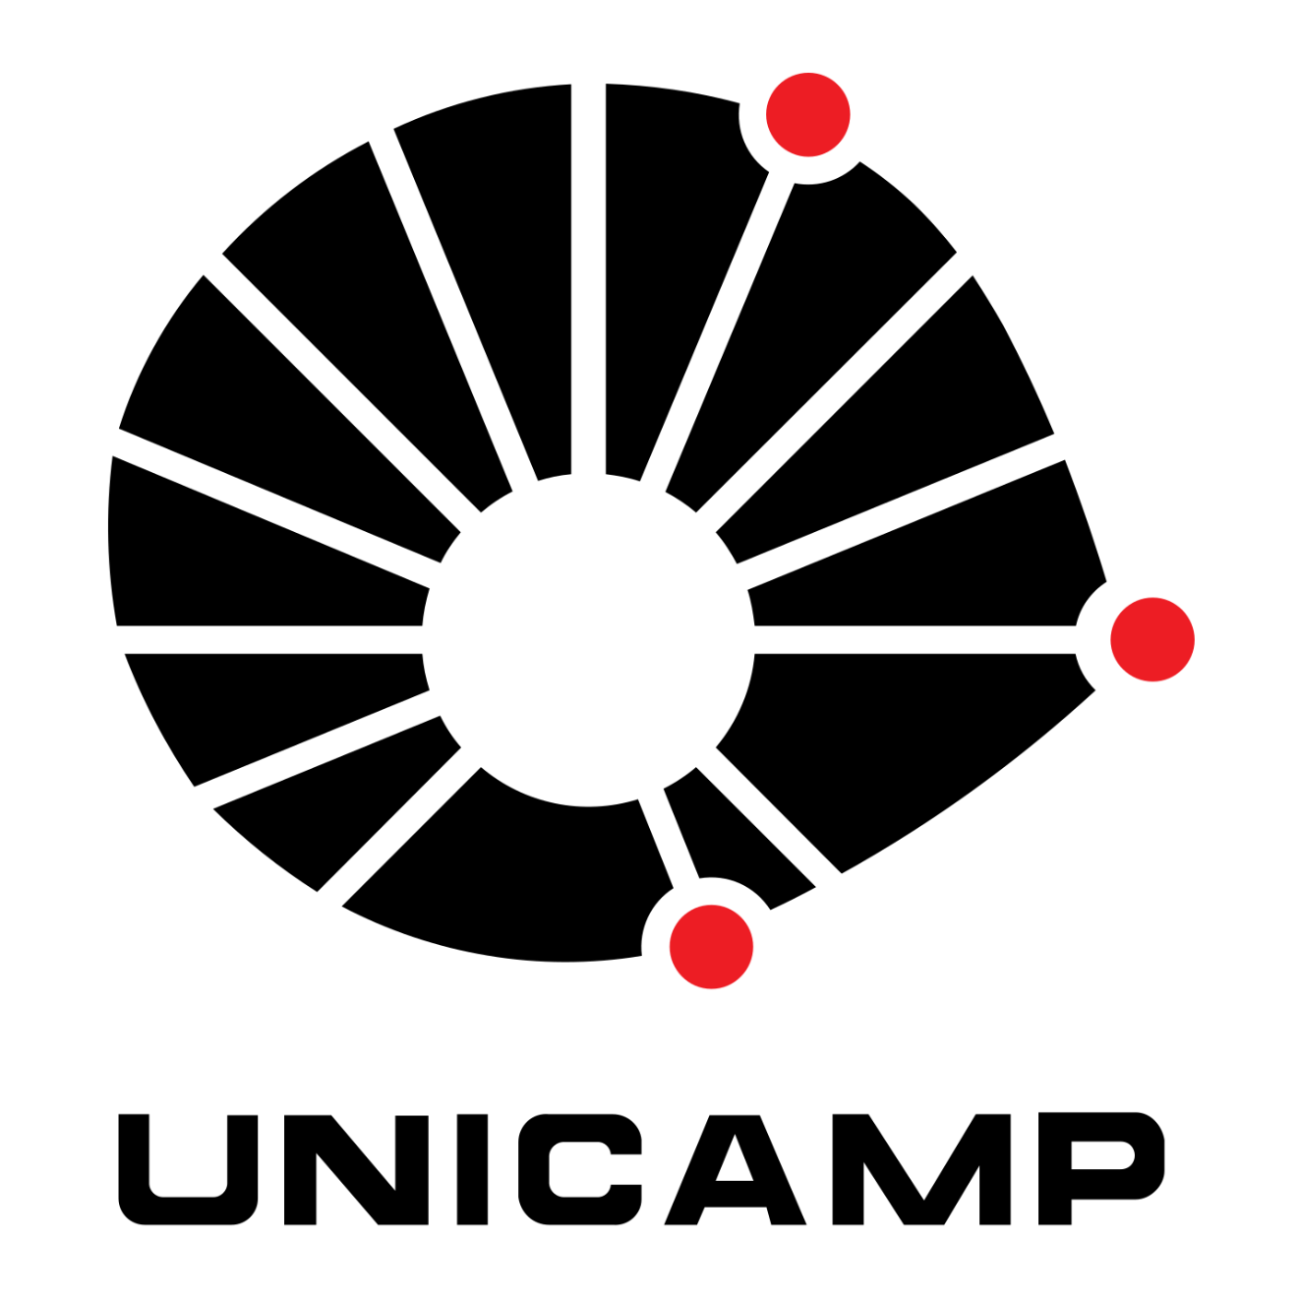
\includegraphics[height=1.1cm]{figures/UNICAMP.png} \hspace{8cm}
    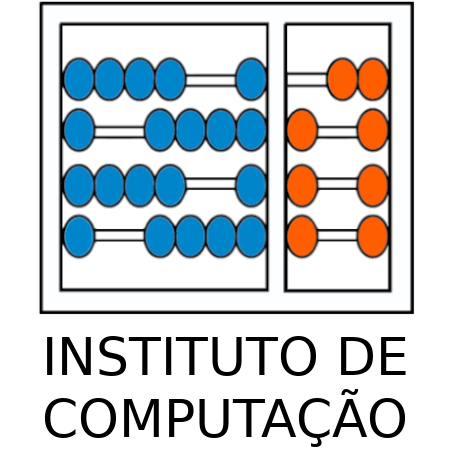
\includegraphics[height=1.1cm]{figures/IC.png}
  \end{center}
  \vspace{-0.2cm}
  \titlepage
\end{frame}

% ==============================================================================
% SEÇÃO: REVISÃO E INTRODUÇÃO
% ==============================================================================
\begin{frame}[plain]
  \centering
  \vspace{2cm}
  {\Huge \textcolor{unicampblue}{\textbf{Revisão e Introdução}}}\\
  \vspace{0.5cm}
  {\large \textcolor{unicampteal}{Do Gargalo do Passo Escalar à Curvatura de 2ª Ordem}}
\end{frame}

% SLIDE 1
\begin{frame}{Da Aula 10: O Que Já Temos}
  \begin{columns}[T]
    \begin{column}{0.48\textwidth}
      \textbf{A Estrutura do SGD:}
      \begin{itemize}
        \item O gradiente estocástico $\mathbf{g}_k = \nabla f_{i_k}(\mathbf{w}_k)$ é um estimador não viesado: $\mathbb{E}[\mathbf{g}_k] = \nabla f(\mathbf{w}_k)$.
        \item O mini-batch $B$ reduz a variância por $\sigma^2/B$ e satura a largura de banda de GPUs.
        \item As condições de Robbins-Monro asseguram convergência assintótica para o mínimo global.
      \end{itemize}
    \end{column}
    \begin{column}{0.48\textwidth}
      \textbf{A Limitação que Restou:}
      \begin{itemize}
        \item O SGD adota uma \textbf{taxa de aprendizado escalar única} $\alpha$ para todos os parâmetros:
        \[\mathbf{w}_{k+1} = \mathbf{w}_k - \alpha \mathbf{g}_k\]
        \item Em paisagens anisotrópicas ($\kappa = \lambda_{\max}/\lambda_{\min} \gg 1$), coordenadas diferentes exigem passos de escalas totalmente distintas!
      \end{itemize}
    \end{column}
  \end{columns}
\end{frame}

% SLIDE 2
\begin{frame}{Ideia Central: Curvatura e Escala}
  \begin{itemize}
    \item O \textbf{Gradiente ($\nabla f$)} é de 1ª ordem: aponta para onde a função sobe com maior taxa instantânea, mas é completamente cego à curvatura do relevo.
    \vspace{0.3cm}
    \item A \textbf{Hessiana ($\nabla^2 f$)} é de 2ª ordem: mede a abertura e a rotação da bacia elíptica em cada direção do espaço de parâmetros.
  \end{itemize}
  \vspace{0.4cm}
  \begin{calloutimportant}[A Pergunta Central]
    Se conhecêssemos a curvatura local exata, qual seria o passo ideal? E quando esse passo for computacionalmente proibitivo ($\mathcal{O}(d^3)$), como aproximá-lo em tempo linear $\mathcal{O}(d)$?
  \end{calloutimportant}
\end{frame}

% SLIDE 3
\begin{frame}{Roteiro da Aula}
  \begin{enumerate}
    \item \textbf{O Modelo Quadrático de Newton:} Dedução analítica via Taylor de 2ª ordem, decremento de Newton e a invariância afim.
    \vspace{0.2cm}
    \item \textbf{As Três Patologias em Larga Escala:} Por que o método puro colapsa em Deep Learning ($\mathcal{O}(d^3)$ de custo, $\mathcal{O}(d^2)$ de memória e armadilhas em pontos de sela).
    \vspace{0.2cm}
    \item \textbf{A Geometria do Precondicionamento:} Como transformar a métrica do espaço e o ponto doce de $\mathcal{O}(d)$ com matrizes diagonais.
    \vspace{0.2cm}
    \item \textbf{Escalas Adaptativas na Prática (AdaGrad e RMSProp):} Construção de taxas adaptativas por coordenada no contexto de SGD usando apenas 1ª ordem.
  \end{enumerate}
\end{frame}

% SLIDE 4
\begin{frame}{Problema Motivador: California Housing}
  \begin{columns}[T]
    \begin{column}{0.48\textwidth}
      \textbf{Atributos com Escalas Díspares:}
      \begin{itemize}
        \item \texttt{MedInc} (renda) varia em dezenas.
        \item \texttt{AveBedrms} varia em frações unitárias.
        \item Hessiana empírica no mínimo:
        \[\lambda_{\max} \approx 6.300, \quad \lambda_{\min} \approx 0{,}27\]
        \[\kappa = \frac{\lambda_{\max}}{\lambda_{\min}} \approx 23.460{,}5\]
      \end{itemize}
    \end{column}
    \begin{column}{0.48\textwidth}
      \textbf{O Dilema do Gradiente:}
      \begin{itemize}
        \item Teto de estabilidade: $\alpha < \frac{2}{\lambda_{\max}} \approx 0{,}0003$.
        \item Contração na direção suave:
        \[\rho = 1 - \alpha \lambda_{\min} \approx 0{,}99991\]
        \item Reduzir o resíduo à metade exige mais de \textbf{7.700 iterações} de descida em lote!
      \end{itemize}
    \end{column}
  \end{columns}
\end{frame}

% SLIDE 5: PAUSA 1
\begin{frame}{Pausa 1: A Limitação do Passo Escalar Único}
  \begin{callouttip}[O Dilema da Taxa Global]
    Suponha uma função quadrática $f(w_1, w_2) = \frac{1}{2}(1000 w_1^2 + w_2^2)$. O que acontece ao aplicar Gradiente Descendente com passo escalar único $\alpha$? Qual é o valor máximo de $\alpha$ para evitar divergência em $w_1$? Sob esse $\alpha$, quantas iterações são necessárias para reduzir o erro em $w_2$ por um fator de 10?
  \end{callouttip}

  \begin{callouttip}[Diagnóstico de Condicionamento]
    \begin{itemize}
      \item[\qmark] Em uma superfície com $\kappa = 1000$, o maior autovalor da Hessiana impõe o teto da taxa de aprendizado admissível ($\alpha < 2/\lambda_{\max}$).
      \item[\qmark] Ao selecionar $\alpha = 1/\lambda_{\max}$, a coordenada de $\lambda_{\min}$ atinge o valor ótimo em 1 única iteração.
      \item[\qmark] A padronização por escore $Z$ elimina todas as discrepâncias de curvatura em modelos não-lineares arbitrários.
      \item[\qmark] Em modelos com dados esparsos, atributos raros recebem gradientes nulos na maioria dos passos; uma taxa escalar pequena retarda seu progresso.
    \end{itemize}
  \end{callouttip}
\end{frame}

% SLIDE 6: PAUSA 1 - RESPOSTA
\begin{frame}{Pausa 1: A Limitação do Passo Escalar Único --- Resposta}
  \begin{callouttip}[Diagnóstico de Condicionamento --- Resposta]
    \begin{itemize}
      \item[\cmark] \textbf{Verdadeiro.} A dinâmica espectral $(I - \alpha H)$ diverge se $|1 - \alpha \lambda_{\max}| \ge 1 \implies \alpha < 2/\lambda_{\max}$.
      \item[\xmark] \textbf{Falso.} Sob $\alpha = 1/\lambda_{\max}$, a coordenada suave contrai por $1 - \frac{1}{\kappa} = 0{,}999$, exigindo milhares de iterações.
      \item[\xmark] \textbf{Falso.} O $Z$-score equaliza apenas as variâncias marginais na entrada; não remove curvaturas cruzadas nem não-linearidades em redes profundas.
      \item[\cmark] \textbf{Verdadeiro.} Gradientes esparsos requerem passos maiores quando ativados, o que é inviabilizado por uma taxa global pequena.
    \end{itemize}
  \end{callouttip}
  \vspace{0.2cm}
  \textbf{Voltando à pergunta:} Para $w_1$, $\alpha < 2/1000 = 0{,}002$. Com $\alpha = 0{,}001$, a contração em $w_2$ é $1 - 0{,}001 \times 1 = 0{,}999$. Para reduzir o erro em $10\times$ ($(0{,}999)^k \le 0{,}1$), são necessárias $\approx \mathbf{2.301}$ iterações!
\end{frame}

% ==============================================================================
% SEÇÃO: INTUIÇÃO
% ==============================================================================
\begin{frame}[plain]
  \centering
  \vspace{2cm}
  {\Huge \textcolor{unicampblue}{\textbf{Intuição Geométrica}}}\\
  \vspace{0.5cm}
  {\large \textcolor{unicampteal}{A Bacia Elíptica e a Lente Métrica}}
\end{frame}

% SLIDE 8
\begin{frame}{A Lente Métrica de Newton}
  \begin{columns}[T]
    \begin{column}{0.48\textwidth}
      \textbf{O Vale Estreito e o GD:}
      \begin{itemize}
        \item Em ravinas elípticas, as paredes laterais são íngremes e a calha é plana.
        \item O gradiente aponta \textbf{quase perpendicularmente à calha}, empurrando o otimizador em ziguezague de parede em parede.
        \item O GD é escravo do sistema de coordenadas euclidiano rígido.
      \end{itemize}
    \end{column}
    \begin{column}{0.48\textwidth}
      \textbf{A Lente Deformadora de Newton:}
      \begin{itemize}
        \item A Hessiana $H = \nabla^2 f(\mathbf{w})$ mede a curvatura direcional exata.
        \item Ao multiplicar por $H^{-1}$, Newton \textbf{esfericiza o espaço}:
        \[\text{Elipses} \;\xrightarrow{\;H^{-1/2}\;}\; \text{Círculos}\]
        \item No espaço deformado, o gradiente aponta \textbf{em linha reta} para o minimizador!
      \end{itemize}
    \end{column}
  \end{columns}
\end{frame}

% SLIDE 9: VISUALIZAÇÃO
\begin{frame}{Visualização: Deformação Métrica em Bacia Elíptica}
  \centering
  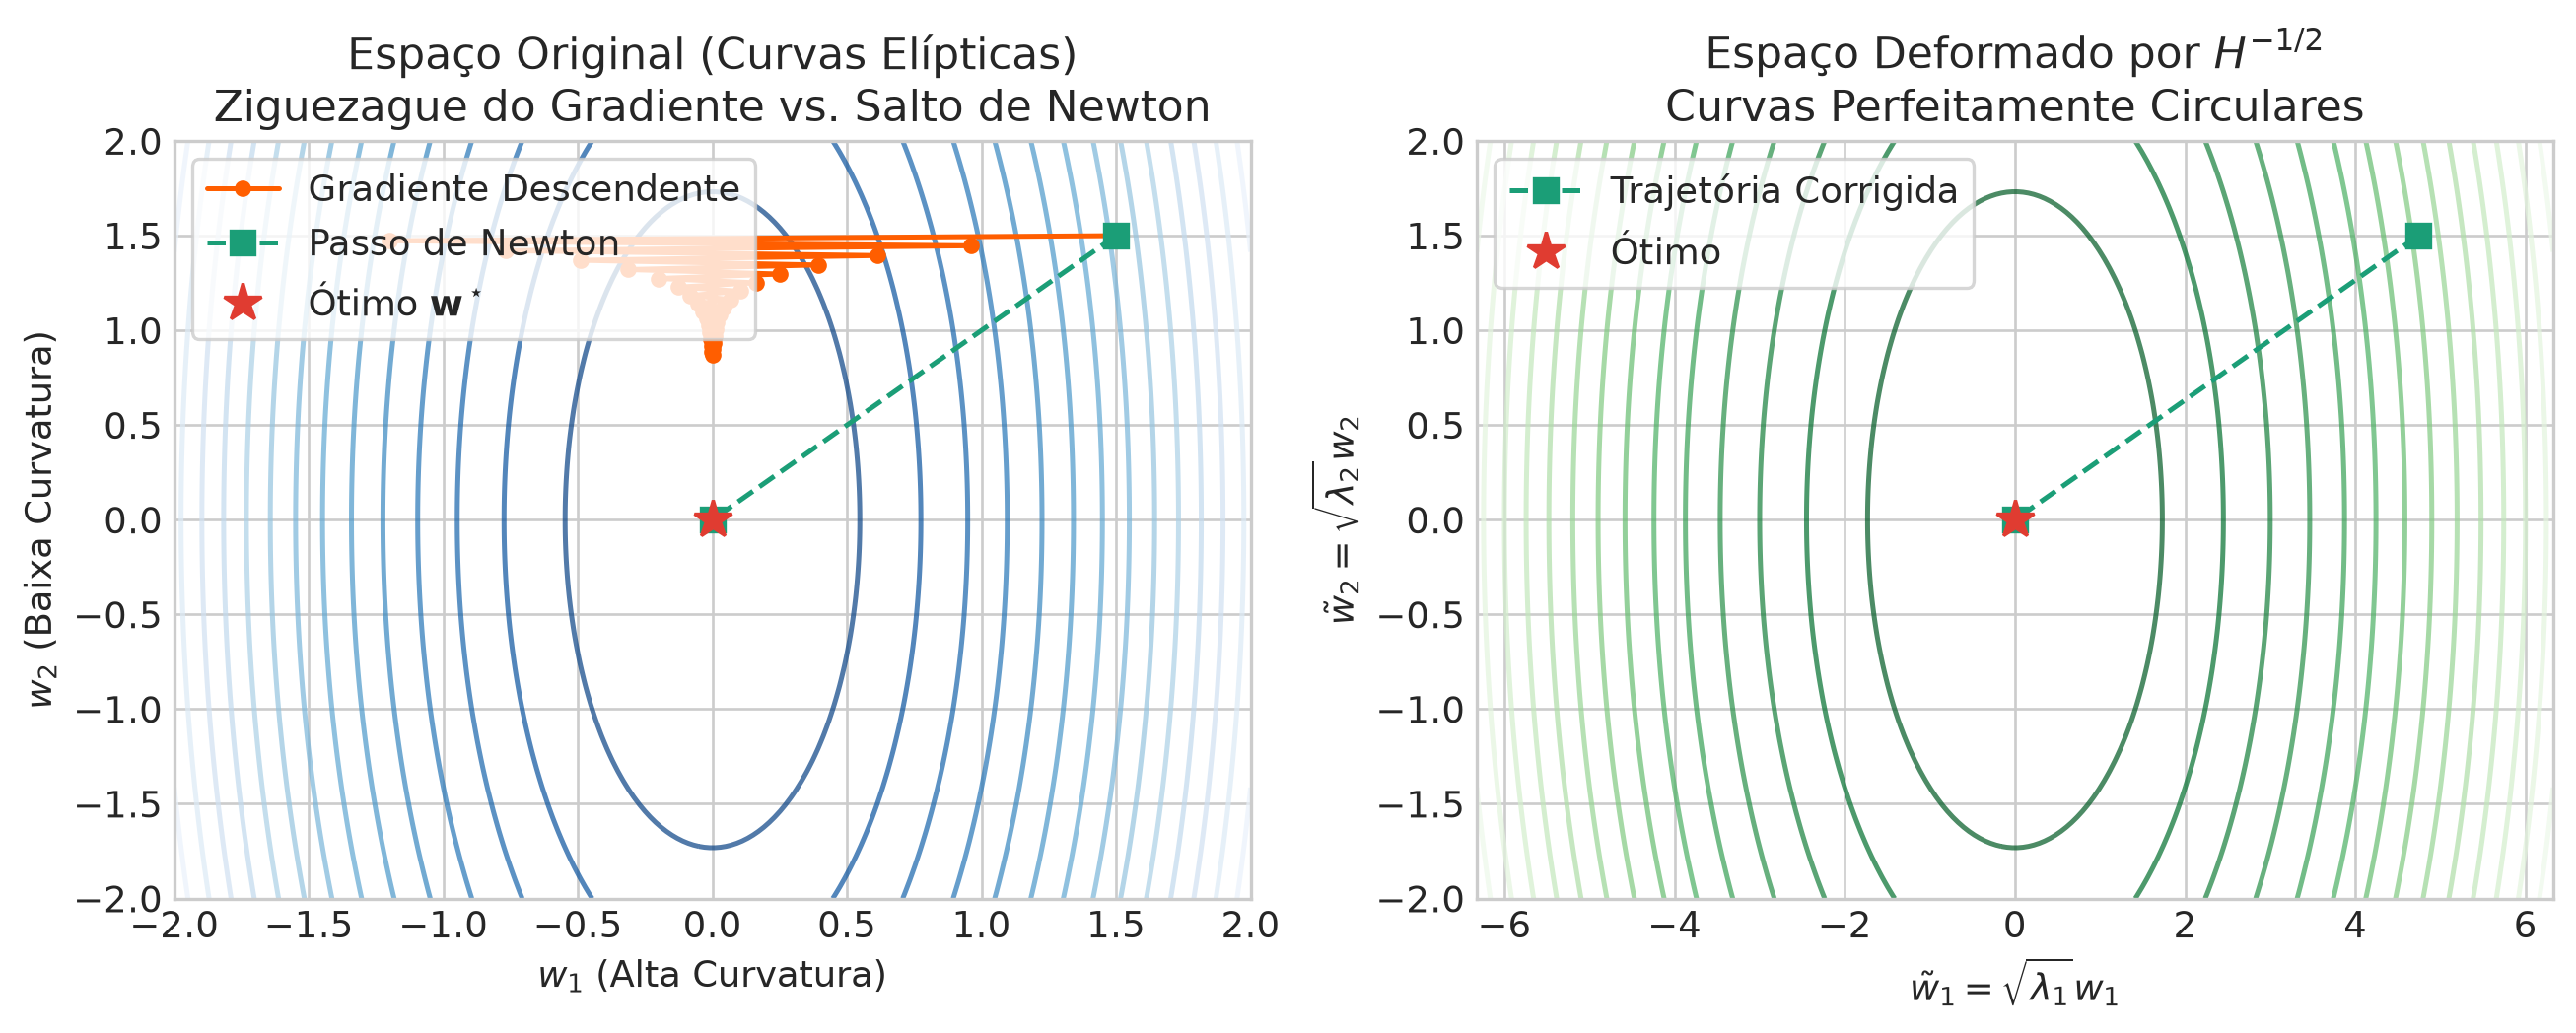
\includegraphics[width=0.88\textwidth]{figures/basin_deformation.png}\\
  \vspace{0.2cm}
  {\footnotesize \textbf{À esquerda:} Curvas de nível elípticas originais ($\kappa = 25$) com ziguezague do GD. \textbf{À direita:} Espaço deformado por $H^{-1/2}$, onde o passo de Newton converge em linha reta.}
\end{frame}

% ==============================================================================
% SEÇÃO: BLOCO 1
% ==============================================================================
\begin{frame}[plain]
  \centering
  \vspace{2cm}
  {\Huge \textcolor{unicampblue}{\textbf{Bloco 1}}}\\
  \vspace{0.5cm}
  {\large \textcolor{unicampteal}{Aproximação Quadrática de Taylor e o Método de Newton}}
\end{frame}

% SLIDE 11
\begin{frame}{Derivação do Passo do Gradiente (Taylor de 1ª Ordem)}
  \textbf{1. Expansão de Taylor com Resto de 2ª Ordem:}
  \[f(\mathbf{w}_k + \Delta\mathbf{w}) = f(\mathbf{w}_k) + \nabla f(\mathbf{w}_k)^T \Delta\mathbf{w} + R_1(\Delta\mathbf{w})\]
  \begin{itemize}
    \item Resto exato: $R_1(\Delta\mathbf{w}) = \frac{1}{2}\Delta\mathbf{w}^T \nabla^2 f(\boldsymbol{\xi})\Delta\mathbf{w}$ (sem o resto, $\inf \nabla f^T \Delta\mathbf{w} = -\infty$).
  \end{itemize}
  \vspace{0.2cm}
  \textbf{2. Penalidade Esférica (Lema da Descida, Aula 8):}
  \[R_1(\Delta\mathbf{w}) \approx \frac{1}{2\alpha}\|\Delta\mathbf{w}\|_2^2 \implies m_{\text{GD}}(\Delta\mathbf{w}) = f(\mathbf{w}_k) + \nabla f^T \Delta\mathbf{w} + \frac{1}{2\alpha}\|\Delta\mathbf{w}\|^2\]
  \vspace{0.2cm}
  \textbf{3. Passo Ótimo:} $\nabla_{\Delta\mathbf{w}} m_{\text{GD}} = \mathbf{0} \implies \Delta\mathbf{w}_{\text{GD}} = -\alpha \nabla f(\mathbf{w}_k)$
  \vspace{0.3cm}
  \begin{calloutwarning}[O Que Falta no Gradiente Descendente?]
    O \textbf{resto de 2ª ordem real}: toda a curvatura anisotrópica foi substituída por uma penalidade esférica isotrópica $\frac{1}{\alpha} I$.
  \end{calloutwarning}
\end{frame}

% SLIDE 12
\begin{frame}{Derivação do Passo de Newton (Taylor de 2ª Ordem)}
  \textbf{1. Expansão de 2ª Ordem com Resto de 3ª Ordem:}
  \[f(\mathbf{w}_k + \Delta\mathbf{w}) = \underbrace{f(\mathbf{w}_k) + \nabla f(\mathbf{w}_k)^T \Delta\mathbf{w} + \frac{1}{2} \Delta\mathbf{w}^T H_k \Delta\mathbf{w}}_{q(\Delta\mathbf{w})} + R_2(\Delta\mathbf{w})\]
  \begin{itemize}
    \item Newton \textbf{incorpora a curvatura real} $H_k = \nabla^2 f(\mathbf{w}_k)$; o novo resto é $R_2 = \mathcal{O}(\|\Delta\mathbf{w}\|^3)$.
  \end{itemize}
  \vspace{0.2cm}
  \textbf{2. Minimizando o Modelo Quadrático $q(\Delta\mathbf{w})$:}
  \[\nabla_{\Delta\mathbf{w}} q(\Delta\mathbf{w}) = \nabla f(\mathbf{w}_k) + H_k \Delta\mathbf{w} = \mathbf{0} \implies \Delta\mathbf{w}_{\text{nt}} = -H_k^{-1} \nabla f(\mathbf{w}_k)\]
  \vspace{0.3cm}
  \begin{calloutnote}[O Que Falta no Método de Newton?]
    O \textbf{resto de 3ª ordem} $R_2 = \mathcal{O}(\|\Delta\mathbf{w}\|^3)$!
    \begin{itemize}
      \item Se $f$ for quadrática $\implies R_2 \equiv 0$ (\textbf{modelo exato em todo $\mathbb{R}^d$, converge em 1 passo!}).
      \item Se $f$ for geral $\implies R_2 \neq 0$ (o passo só é confiável onde $\|\Delta\mathbf{w}\|^3 \ll \|\Delta\mathbf{w}\|^2$).
    \end{itemize}
  \end{calloutnote}
\end{frame}

% SLIDE 13
\begin{frame}{A Regra de Atualização e a Auto-Calibração de Escala}
  \textbf{1. Translação pelo Passo Ótimo:}
  \[\mathbf{w}_{k+1} \triangleq \mathbf{w}_k + \Delta\mathbf{w}_{\text{nt}} = \mathbf{w}_k - [\nabla^2 f(\mathbf{w}_k)]^{-1} \nabla f(\mathbf{w}_k)\]
  \vspace{0.3cm}
  \textbf{2. Análise Dimensional: Por que Newton Dispensa $\alpha$?}
  \[[H_k^{-1} \nabla f] = \underbrace{\frac{[\text{param}]^2}{[\text{perda}]}}_{[H^{-1}]} \times \underbrace{\frac{[\text{perda}]}{[\text{param}]}}_{[\nabla f]} = [\text{param}]\]
  \begin{itemize}
    \item O GD precisa de $\alpha$ para converter inclinação em distância.
    \item Em Newton, $H^{-1}$ já calcula analiticamente a distância física exata até o fundo da bacia!
  \end{itemize}
\end{frame}

% SLIDE 14
\begin{frame}{Como Surge o Decremento de Newton?}
  \textbf{A Pergunta:} Quanto o modelo $q(\Delta\mathbf{w})$ promete que a perda vai diminuir com o passo $\Delta\mathbf{w}_{\text{nt}} = -H_k^{-1}\mathbf{g}_k$?
  \vspace{0.2cm}
  \textbf{Avaliando o modelo no vértice da parábola:}
  \[q(\Delta\mathbf{w}_{\text{nt}}) = f(\mathbf{w}_k) - \mathbf{g}_k^T H_k^{-1}\mathbf{g}_k + \frac{1}{2}\mathbf{g}_k^T H_k^{-1}\mathbf{g}_k = f(\mathbf{w}_k) - \frac{1}{2}\mathbf{g}_k^T H_k^{-1}\mathbf{g}_k\]
  \vspace{0.3cm}
  \begin{calloutimportant}[A Redução Prevista no Custo]
    \[f(\mathbf{w}_k) - q(\Delta\mathbf{w}_{\text{nt}}) = \frac{1}{2} \mathbf{g}_k^T H_k^{-1} \mathbf{g}_k \triangleq \frac{1}{2} \lambda(\mathbf{w})^2\]
    A quantidade $\lambda(\mathbf{w})^2 = \mathbf{g}_k^T H_k^{-1} \mathbf{g}_k$ mede exatamente o dobro da descida prevista pelo modelo quadrático!
  \end{calloutimportant}
\end{frame}

% SLIDE 15
\begin{frame}{O Decremento de Newton: Interpretação e Parada}
  \textbf{Definição do Decremento de Newton $\lambda(\mathbf{w})$:}
  \[\lambda(\mathbf{w}) \triangleq \sqrt{\mathbf{g}^T H^{-1} \mathbf{g}} \implies f(\mathbf{w}) - q(\Delta\mathbf{w}_{\text{nt}}) = \frac{1}{2}\lambda(\mathbf{w})^2\]
  \vspace{0.2cm}
  \textbf{Interpretações Geométricas:}
  \begin{itemize}
    \item \textbf{Norma do gradiente na métrica da curvatura:} $\lambda(\mathbf{w}) = \|\nabla f(\mathbf{w})\|_{H^{-1}}$.
    \item \textbf{Comprimento ponderado do passo:} $\|\Delta\mathbf{w}_{\text{nt}}\|_H = \sqrt{\Delta\mathbf{w}^T H \Delta\mathbf{w}} = \lambda(\mathbf{w})$.
    \item \textbf{Derivada direcional ao longo do passo:} $\nabla f^T \Delta\mathbf{w}_{\text{nt}} = -\lambda(\mathbf{w})^2$.
  \end{itemize}
  \vspace{0.2cm}
  \begin{callouttip}[Critério de Parada Rigoroso (Boyd §9.5.3)]
    Sob forte convexidade, $f(\mathbf{w}) - f(\mathbf{w}^\star) \le \frac{1}{2\mu}\lambda(\mathbf{w})^2$.
    O algoritmo encerra com segurança teórica quando $\frac{1}{2}\lambda(\mathbf{w})^2 \le \epsilon$.
  \end{callouttip}
\end{frame}

% SLIDE 16
\begin{frame}{Invariância Afim de Newton}
  \textbf{Mudança Linear de Coordenadas:} $\tilde{\mathbf{w}} = A \mathbf{w}$ ($A$ inversível), $\phi(\tilde{\mathbf{w}}) = f(A^{-1}\tilde{\mathbf{w}})$.
  \begin{itemize}
    \item Gradiente transformado: $\nabla \phi = A^{-T} \nabla f$
    \item Hessiana transformada: $\nabla^2 \phi = A^{-T} \nabla^2 f A^{-1}$
  \end{itemize}
  \vspace{0.2cm}
  \textbf{O Passo de Newton no Novo Espaço:}
  \[\Delta\tilde{\mathbf{w}}_{\text{nt}} = -[\nabla^2 \phi]^{-1} \nabla \phi = -[A (\nabla^2 f)^{-1} A^T] A^{-T} \nabla f = A \Delta\mathbf{w}_{\text{nt}}\]
  \vspace{0.2cm}
  \begin{calloutnote}[Retorno ao Espaço Original]
    \[A^{-1}\Delta\tilde{\mathbf{w}}_{\text{nt}} = A^{-1}(A \Delta\mathbf{w}_{\text{nt}}) = \Delta\mathbf{w}_{\text{nt}}\]
    A trajetória de Newton é \textbf{rigorosamente invariante} para qualquer matriz inversível $A$ (escalas, rotações ou cisalhamentos).
  \end{calloutnote}
\end{frame}

% SLIDE 17
\begin{frame}{Por Que o Gradiente Descendente Quebra sob Escala?}
  \textbf{Passo de GD no espaço transformado $\tilde{\mathbf{w}}$:}
  \[\Delta\tilde{\mathbf{w}}_{\text{GD}} = -\alpha \nabla_{\tilde{\mathbf{w}}} \phi = -\alpha A^{-T} \nabla_{\mathbf{w}} f(\mathbf{w})\]
  \vspace{0.2cm}
  \textbf{Mapeando de volta para o espaço original ($A^{-1}\Delta\tilde{\mathbf{w}}$):}
  \[\Delta\mathbf{w}_{\text{equiv}} = A^{-1}(-\alpha A^{-T} \nabla f) = -\alpha (A^T A)^{-1} \nabla f(\mathbf{w})\]
  \vspace{0.2cm}
  \textbf{O Contraste Fundamental:}
  \[\Delta\mathbf{w}_{\text{equiv}} = -\alpha (A^T A)^{-1} \nabla f \;\neq\; -\alpha \nabla f\]
  \begin{itemize}
    \item Só coincide com o GD original se $(A^T A)^{-1} = I \iff A^T A = I$ (\textbf{matriz ortogonal / rotação pura}).
  \end{itemize}
  \vspace{0.2cm}
  \begin{calloutwarning}[Conclusão Prática]
    Se $A = \text{diag}(100, 1)$, a trajetória do GD deforma-se por $(A^T A)^{-1}$. O GD é \textbf{escravo das unidades}; Newton é \textbf{afim-invariante}!
  \end{calloutwarning}
\end{frame}

% SLIDE 18
\begin{frame}{Por Que a Invariância Afim É Crucial na Prática?}
  \textbf{1. Imunidade à Escala das Variáveis (\texttt{StandardScaler}):}
  \begin{itemize}
    \item \textbf{No GD:} Misturar metros e milímetros explode $\kappa$ para $10^6$ $\implies$ z-score é muleta obrigatória.
    \item \textbf{Em Newton:} Com ou sem normalização, a trajetória e os passos físicos são \textbf{rigorosamente idênticos}!
  \end{itemize}
  \vspace{0.2cm}
  \textbf{2. Imunidade a Correlações entre Variáveis:}
  \begin{itemize}
    \item Features correlacionadas geram ravinas elípticas rotacionadas e ziguezague no GD.
    \item As derivadas mistas $\frac{\partial^2 f}{\partial w_i \partial w_j}$ de $H$ cancelam a rotação e caminham direto ao vértice.
  \end{itemize}
  \vspace{0.3cm}
  \begin{callouttip}[A Ponte Conceitual para o Precondicionamento]
    Newton tem invariância afim completa ($\mathcal{O}(d^3)$); o GD tem zero ($\mathcal{O}(d)$).\\
    O \textbf{Precondicionamento Diagonal} busca resgatar a invariância sob escalas a custo linear $\mathcal{O}(d)$!
  \end{callouttip}
\end{frame}

% SLIDE 19: PAUSA 2
\begin{frame}{Pausa 2: O Passo de Newton e a Invariância Afim}
  \begin{callouttip}[O Salto em Formas Quadráticas]
    Seja $f(\mathbf{w}) = \frac{1}{2}\mathbf{w}^T A \mathbf{w} - \mathbf{b}^T \mathbf{w}$ com $A \succ 0$. Quantas iterações o Método de Newton exige para encontrar a solução exata $\mathbf{w}^\star = A^{-1}\mathbf{b}$ partindo de um $\mathbf{w}_0$ arbitrário? Qual é o papel geométrico do decremento de Newton $\lambda(\mathbf{w})^2$?
  \end{callouttip}

  \begin{callouttip}[Propriedades de Segunda Ordem]
    \begin{itemize}
      \item[\qmark] Se $f$ for uma forma quadrática estritamente convexa, a expansão de Taylor de 2ª ordem é exata, tornando o resíduo superior nulo.
      \item[\qmark] O passo de Newton $\Delta\mathbf{w}_{\text{nt}} = -H^{-1}\nabla f$ tem unidade dimensional compatível com o parâmetro $\mathbf{w}$.
      \item[\qmark] Ao transformar $\mathbf{w} \to c \mathbf{w}$ ($c > 0$), o passo do GD clássico é multiplicado por $1/c$, preservando a mesma trajetória.
      \item[\qmark] O decremento $\lambda(\mathbf{w})^2 = \nabla f^T H^{-1} \nabla f$ é estritamente não-negativo para $H \succ 0$ e anula-se sse $\nabla f = \mathbf{0}$.
    \end{itemize}
  \end{callouttip}
\end{frame}

% SLIDE 20: PAUSA 2 - RESPOSTA
\begin{frame}{Pausa 2: O Passo de Newton e a Invariância Afim --- Resposta}
  \begin{callouttip}[Propriedades de Segunda Ordem --- Resposta]
    \begin{itemize}
      \item[\cmark] \textbf{Verdadeiro.} Derivadas de ordem 3+ são identicamente nulas; o paraboloide de Taylor coincide perfeitamente com a função real.
      \item[\cmark] \textbf{Verdadeiro.} $[H^{-1}\nabla f] = \frac{[\text{param}]^2}{[\text{perda}]} \times \frac{[\text{perda}]}{[\text{param}]} = [\text{param}]$, tornando o passo auto-escalado.
      \item[\xmark] \textbf{Falso.} O gradiente transforma por $1/c$, mas o passo euclidiano precisaria escalar por $c$; o GD quebra a equivalência física.
      \item[\cmark] \textbf{Verdadeiro.} Como $H \succ 0 \implies H^{-1} \succ 0$, a forma quadrática é nula se e somente se o gradiente for o vetor nulo.
    \end{itemize}
  \end{callouttip}
  \vspace{0.2cm}
  \textbf{Voltando à pergunta:} Exatamente \textbf{1 iteração}! Pois $H_0 = A$ e $\nabla f(\mathbf{w}_0) = A \mathbf{w}_0 - \mathbf{b}$, de modo que $\mathbf{w}_1 = \mathbf{w}_0 - A^{-1}(A \mathbf{w}_0 - \mathbf{b}) = A^{-1}\mathbf{b} = \mathbf{w}^\star$.
\end{frame}

% ==============================================================================
% SEÇÃO: BLOCO 2
% ==============================================================================
\begin{frame}[plain]
  \centering
  \vspace{2cm}
  {\Huge \textcolor{unicampblue}{\textbf{Bloco 2}}}\\
  \vspace{0.5cm}
  {\large \textcolor{unicampteal}{As Três Patologias de Newton em Aprendizado de Máquina}}
\end{frame}

% SLIDE 22
\begin{frame}{As Três Patologias de Newton}
  \begin{columns}[T]
    \begin{column}{0.32\textwidth}
      \textbf{1. O Muro Cúbico $\mathcal{O}(d^3)$}
      \begin{itemize}
        \item Resolver $H \Delta\mathbf{w} = -\mathbf{g}$ via Cholesky custa $\frac{1}{3}d^3$ FLOPs.
        \item Memória: armazenar $H \in \mathbb{R}^{d \times d}$ exige $\mathcal{O}(d^2)$.
        \item Para $d = 10^9$ (LLMs): $4 \times 10^{18}$ bytes (4 Exabytes!).
      \end{itemize}
    \end{column}
    \begin{column}{0.32\textwidth}
      \textbf{2. Terrenos Não-Convexos}
      \begin{itemize}
        \item Se $H$ possuir autovalores negativos ($\lambda_i < 0$), o modelo quadrático é ilimitado inferiormente.
        \item O passo pode apontar para um \textbf{máximo local} ou ser atraído por \textbf{pontos de sela}!
      \end{itemize}
    \end{column}
    \begin{column}{0.32\textwidth}
      \textbf{3. Ruído de Mini-Batch}
      \begin{itemize}
        \item Avaliar $H$ completa custa $\mathcal{O}(Nd^2)$.
        \item Em lote $B < d$, a Hessiana amostral $\hat{H}$ tem posto $\le B$ (é singular!).
        \item Autovalores próximos de zero amplificam o ruído por $1/\hat{\lambda}_i$.
      \end{itemize}
    \end{column}
  \end{columns}
\end{frame}

% SLIDE 23
\begin{frame}{Regularização de Levenberg-Marquardt}
  \textbf{Sistema Linear Modificado (Newton Amortecido):}
  \[(H_k + \lambda_k I)\Delta\mathbf{w} = -\nabla f(\mathbf{w}_k), \quad \text{com } \lambda_k > 0\]
  \vspace{0.2cm}
  \textbf{Espectro dos Autovalores:}
  \[\lambda_i(H_k + \lambda_k I) = \lambda_i(H_k) + \lambda_k\]
  Basta escolher $\lambda_k > |\lambda_{\min}|$ para garantir que a matriz seja estritamente positiva definida!
  \vspace{0.2cm}
  \textbf{Interpolação Suave:}
  \[\lambda_k \to 0 \implies \text{Newton Puro} \qquad\Longleftrightarrow\qquad \lambda_k \to \infty \implies \text{Gradiente Descendente}\]
  \vspace{0.3cm}
  \begin{calloutwarning}[Limitação Persistente]
    Resolve a indefinição de sinal, mas \textbf{ainda custa $\mathcal{O}(d^3)$} para resolver o sistema linear a cada iteração!
  \end{calloutwarning}
\end{frame}

% SLIDE 24: PAUSA 3
\begin{frame}{Pausa 3: Patologias de Newton em Alta Dimensão}
  \begin{callouttip}[O Salto no Ponto de Sela]
    Considere a função hiperbólica $f(w_1, w_2) = w_1^2 - w_2^2$, que possui um ponto de sela em $(0, 0)$. Calcule o passo de Newton a partir de $\mathbf{w}_0 = (1, 1)^T$. Para onde o algoritmo se desloca? O que ocorreria se o ponto inicial fosse $(0, 1)^T$?
  \end{callouttip}

  \begin{callouttip}[Escala Computacional de Newton]
    \begin{itemize}
      \item[\qmark] Em problemas não convexos onde a Hessiana é indefinida, o passo de Newton puro pode apontar numa direção de subida da perda.
      \item[\qmark] O custo de memória para armazenar a matriz Hessiana de um modelo com $d = 10^5$ parâmetros em float32 é de aproximadamente $40$ Megabytes.
      \item[\qmark] A regularização de Levenberg-Marquardt garante $H + \lambda I \succ 0$ e reduz a complexidade temporal para $\mathcal{O}(d)$.
      \item[\qmark] Quando estimada em um mini-batch de tamanho $B < d$, a matriz Hessiana amostral é garantidamente singular, com posto no máximo $B$.
    \end{itemize}
  \end{callouttip}
\end{frame}

% SLIDE 25: PAUSA 3 - RESPOSTA
\begin{frame}{Pausa 3: Patologias de Newton em Alta Dimensão --- Resposta}
  \begin{callouttip}[Escala Computacional de Newton --- Resposta]
    \begin{itemize}
      \item[\cmark] \textbf{Verdadeiro.} Se $\lambda_i < 0$, o passo $\Delta w_i = -g_i/\lambda_i$ possui o mesmo sinal de $g_i$, caminhando na direção ascendente!
      \item[\xmark] \textbf{Falso.} $(10^5)^2 \times 4\text{ bytes} = 10^{10} \times 4 = 40\text{ Gigabytes}$, e não Megabytes.
      \item[\xmark] \textbf{Falso.} Levenberg-Marquardt garante positividade, mas resolver o sistema linear ainda exige $\mathcal{O}(d^3)$ FLOPs.
      \item[\cmark] \textbf{Verdadeiro.} A Hessiana da perda empírica em um lote de $B$ amostras é a soma de $B$ matrizes de posto 1, logo $\text{posto} \le B < d$.
    \end{itemize}
  \end{callouttip}
  \vspace{0.2cm}
  \textbf{Voltando à pergunta:} $\nabla f = [2w_1, -2w_2]^T$ e $H = \text{diag}(2, -2)$. O passo é $\Delta\mathbf{w} = -H^{-1}\nabla f = [-1, 1]^T \implies \mathbf{w}_1 = (0, 2)^T$. O algoritmo salta diretamente em direção ao infinito negativo ao longo do eixo $w_2$, divergindo!
\end{frame}

% ==============================================================================
% SEÇÃO: BLOCO 3
% ==============================================================================
\begin{frame}[plain]
  \centering
  \vspace{2cm}
  {\Huge \textcolor{unicampblue}{\textbf{Bloco 3}}}\\
  \vspace{0.5cm}
  {\large \textcolor{unicampteal}{A Geometria do Precondicionamento e a Matriz Diagonal}}
\end{frame}

% SLIDE 27
\begin{frame}{A Geometria do Precondicionamento: Esfericização}
  \textbf{1. Por que Deformar o Espaço?}
  \begin{itemize}
    \item Sob mudança linear $\tilde{\mathbf{w}} = M\mathbf{w}$, a nova Hessiana passa a ser $M^{-T} H M^{-1}$.
    \item Para que o terreno se torne esférico e isotrópico ($M^{-T} H M^{-1} \approx I$):
    \[H \approx M^T M\]
  \end{itemize}
  \vspace{0.2cm}
  \textbf{2. A Escolha da Métrica $M = P^{1/2}$:}
  \begin{itemize}
    \item Seja $P \approx H$ simétrica estritamente positiva definida ($P \succ 0$).
    \item Pela raiz simétrica (Teorema Espectral): escolhemos $M = P^{1/2}$ ($M^T M = P^{1/2} P^{1/2} = P$).
  \end{itemize}
  \vspace{0.2cm}
  \textbf{3. O Gradiente no Espaço Deformado:}
  \[\tilde{\mathbf{w}} = P^{1/2} \mathbf{w} \iff \mathbf{w} = P^{-1/2} \tilde{\mathbf{w}} \implies \nabla_{\tilde{\mathbf{w}}} \phi(\tilde{\mathbf{w}}) = P^{-1/2} \nabla f(\mathbf{w})\]
\end{frame}

% SLIDE 28
\begin{frame}{O Passo Precondicionado Universal}
  \textbf{1. Passo no Espaço Esférico revertido ao Espaço Original:}
  \[\Delta\tilde{\mathbf{w}} = -\alpha \nabla_{\tilde{\mathbf{w}}} \phi = -\alpha P^{-1/2} \nabla f(\mathbf{w})\]
  \[\Delta\mathbf{w} = P^{-1/2} \Delta\tilde{\mathbf{w}} = -\alpha \underbrace{P^{-1/2} P^{-1/2}}_{= P^{-1}} \nabla f(\mathbf{w})\]
  \begin{itemize}
    \item O 1º $P^{-1/2}$ vem da \textbf{regra da cadeia}; o 2º vem da \textbf{mudança de base inversa}.
  \end{itemize}
  \vspace{0.3cm}
  \begin{calloutnote}[Regra Precondicionada Universal: $\mathbf{w}_{k+1} = \mathbf{w}_k - \alpha P^{-1} \nabla f(\mathbf{w}_k)$]
    \begin{itemize}
      \item $P = I \implies$ Gradiente Descendente euclidiano clássico ($\mathcal{O}(d)$)
      \item $P = H \implies$ Método de Newton com $\alpha = 1$ ($\mathcal{O}(d^3)$)
      \item $P = D \implies$ \textbf{Precondicionamento Diagonal} ($\mathcal{O}(d)$!)
    \end{itemize}
  \end{calloutnote}
\end{frame}

% SLIDE 29
\begin{frame}{O Ponto Doce: Precondicionamento Diagonal}
  \begin{columns}[T]
    \begin{column}{0.48\textwidth}
      \textbf{Estrutura Diagonal:}
      \[D = \text{diag}(s_1, s_2, \dots, s_d) \succ 0\]
      \begin{itemize}
        \item Inversão analítica imediata:
        \[D^{-1} = \text{diag}\left(\frac{1}{s_1}, \dots, \frac{1}{s_d}\right)\]
        \item Memória: apenas $d$ escalares ($\mathcal{O}(d)$).
        \item FLOPs: $d$ divisões por passo ($\mathcal{O}(d)$).
      \end{itemize}
    \end{column}
    \begin{column}{0.48\textwidth}
      \textbf{Atualização por Coordenada:}
      \[w_{i, k+1} = w_{i, k} - \frac{\alpha}{s_{i, k}} g_{i, k}\]
      \begin{itemize}
        \item Cada parâmetro $i$ possui sua própria taxa de aprendizado efetiva:
        \[\alpha_i^{\text{eff}} = \frac{\alpha}{s_i}\]
        \item Coordenadas íngremes são atenuadas; coordenadas planas são aceleradas!
      \end{itemize}
    \end{column}
  \end{columns}
\end{frame}

% SLIDE 30: PAUSA 4
\begin{frame}{Pausa 4: Precondicionamento Diagonal}
  \begin{callouttip}[O Desacoplamento Matricial]
    Mostre algebricamente por que a multiplicação matriz-vetor $D^{-1}\mathbf{g}$ com $D = \text{diag}(s_1, \dots, s_d)$ possui custo computacional linear $\mathcal{O}(d)$. Por que essa operação pode ser distribuída perfeitamente em threads paralelas em uma GPU?
  \end{callouttip}

  \begin{callouttip}[Propriedades do Precondicionamento]
    \begin{itemize}
      \item[\qmark] O precondicionamento diagonal equivale a reescalonar cada coordenada $w_i$ por $\sqrt{s_i}$ independentemente.
      \item[\qmark] Uma matriz diagonal é capaz de rotacionar os eixos de coordenadas para cancelar correlações cruzadas da Hessiana.
      \item[\qmark] Se escolhermos $s_i = \frac{\partial^2 f}{\partial w_i^2}$, recuperamos o método de Newton unidimensional aplicado a cada parâmetro.
      \item[\qmark] O custo de memória de armazenar um precondicionador diagonal cresce quadraticamente com a dimensão ($\mathcal{O}(d^2)$).
    \end{itemize}
  \end{callouttip}
\end{frame}

% SLIDE 31: PAUSA 4 - RESPOSTA
\begin{frame}{Pausa 4: Precondicionamento Diagonal --- Resposta}
  \begin{callouttip}[Propriedades do Precondicionamento --- Resposta]
    \begin{itemize}
      \item[\cmark] \textbf{Verdadeiro.} $\tilde{w}_i = \sqrt{s_i} w_i \implies \frac{\partial f}{\partial \tilde{w}_i} = \frac{1}{\sqrt{s_i}} \frac{\partial f}{\partial w_i}$; o passo resultante é $w_i - \frac{\alpha}{s_i} g_i$.
      \item[\xmark] \textbf{Falso.} Matrizes diagonais realizam apenas estiramentos axiais; não rotacionam eixos nem eliminam termos fora da diagonal.
      \item[\cmark] \textbf{Verdadeiro.} É a chamada aproximação de Newton Diagonal, descartando derivadas mistas $\partial^2 f / \partial w_i \partial w_j$.
      \item[\xmark] \textbf{Falso.} O armazenamento é estritamente linear $\mathcal{O}(d)$ (um único vetor com as $d$ entradas diagonais).
    \end{itemize}
  \end{callouttip}
  \vspace{0.2cm}
  \textbf{Voltando à pergunta:} $D^{-1}\mathbf{g} = [g_1/s_1, \dots, g_d/s_d]^T$. Trata-se de um produto Hadamard (elemento a elemento), onde cada coordenada $i$ opera sem consultar nenhuma outra coordenada $j \neq i$. Isso permite que cada thread de GPU execute uma divisão escalar isolada sem barreiras de sincronização!
\end{frame}

% ==============================================================================
% SEÇÃO: BLOCO 4
% ==============================================================================
\begin{frame}[plain]
  \centering
  \vspace{2cm}
  {\Huge \textcolor{unicampblue}{\textbf{Bloco 4}}}\\
  \vspace{0.5cm}
  {\large \textcolor{unicampteal}{Escalas Adaptativas na Prática: AdaGrad e RMSProp}}
\end{frame}

% SLIDE 33
\begin{frame}{Escalas Adaptativas no Contexto de SGD}
  \textbf{1. O Cenário Real: Otimização Estocástica (SGD)}
  \begin{itemize}
    \item No aprendizado supervisionado, operamos quase sempre com \textbf{mini-batches} ($B_t$).
    \item O gradiente observado $\mathbf{g}_t = \nabla f_{B_t}(\mathbf{w}_t)$ possui alto ruído estatístico.
  \end{itemize}
  \vspace{0.2cm}
  \textbf{2. A Extrema Instabilidade de 2ª Ordem no SGD:}
  \begin{itemize}
    \item \textbf{Variância extrema:} A Hessiana varia drasticamente entre lotes sucessivos.
    \item \textbf{Curvatura negativa espúria:} O ruído amostral gera $s_i < 0$, que faria o passo subir a perda!
    \item \textbf{Custo proibitivo:} Diferenciação de 2ª ordem por lote degrada o throughput em GPUs.
  \end{itemize}
  \vspace{0.3cm}
  \begin{callouttip}[A Solução de AdaGrad e RMSProp]
    Nascem \textbf{dentro do SGD}: usam a energia das \textbf{primeiras derivadas} ($g_{t, i}^2$) como proxy empírico da escala local, contornando a instabilidade de 2ª ordem a custo linear $\mathcal{O}(d)$!
  \end{callouttip}
\end{frame}

% SLIDE 34
\begin{frame}{Otimizador AdaGrad (Duchi et al., 2011)}
  \textbf{Intuição:} Acumular a energia dos gradientes estocásticos passados ($g_{\tau, i}^2$) para calibrar a escala por coordenada em dados esparsos.
  \vspace{0.2cm}
  \textbf{Acumulador de Energia:}
  \[G_{t, i} = G_{t-1, i} + g_{t, i}^2 = \sum_{\tau=1}^t g_{\tau, i}^2\]
  \vspace{0.2cm}
  \textbf{Regra de Atualização:}
  \[\mathbf{w}_{t+1} = \mathbf{w}_t - \frac{\alpha}{\sqrt{\mathbf{G}_t} + \epsilon} \odot \mathbf{g}_t\]
  \vspace{0.3cm}
  \begin{calloutwarning}[A Patologia do Congelamento Prematuro]
    $g^2 \ge 0 \implies G_t$ cresce monotonamente. A taxa de aprendizado efetiva $\frac{\alpha}{\sqrt{G_t}}$ decai irreversivelmente para zero, congelando o treinamento antes da convergência em redes profundas!
  \end{calloutwarning}
\end{frame}

% SLIDE 35
\begin{frame}{Otimizador RMSProp (Hinton, 2012)}
  \textbf{Cura do Congelamento:} Substituir a soma infinita por Média Móvel Exponencial (EMA).
  \vspace{0.2cm}
  \textbf{Rastreamento do Segundo Momento Não-Central:}
  \[v_{t, i} = \beta_2 v_{t-1, i} + (1 - \beta_2) g_{t, i}^2, \quad \beta_2 \in [0{,}9, 0{,}99]\]
  \vspace{0.2cm}
  \textbf{Regra de Atualização:}
  \[\mathbf{w}_{t+1} = \mathbf{w}_t - \frac{\alpha}{\sqrt{\mathbf{v}_t} + \epsilon} \odot \mathbf{g}_t\]
  \vspace{0.3cm}
  \begin{calloutnote}[Vantagens]
    \begin{itemize}
      \item Memória temporal efetiva de $\approx \frac{1}{1-\beta_2}$ iterações.
      \item Se o gradiente diminuir, $v_t$ decresce e o passo efetivo \textbf{aumenta}.
      \item Nunca congela prematuramente: tornou-se a espinha dorsal de otimizadores em Deep Learning!
    \end{itemize}
  \end{calloutnote}
\end{frame}

% SLIDE 36: VISUALIZAÇÃO
\begin{frame}{Dinâmica Comparada: AdaGrad vs. RMSProp}
  \centering
  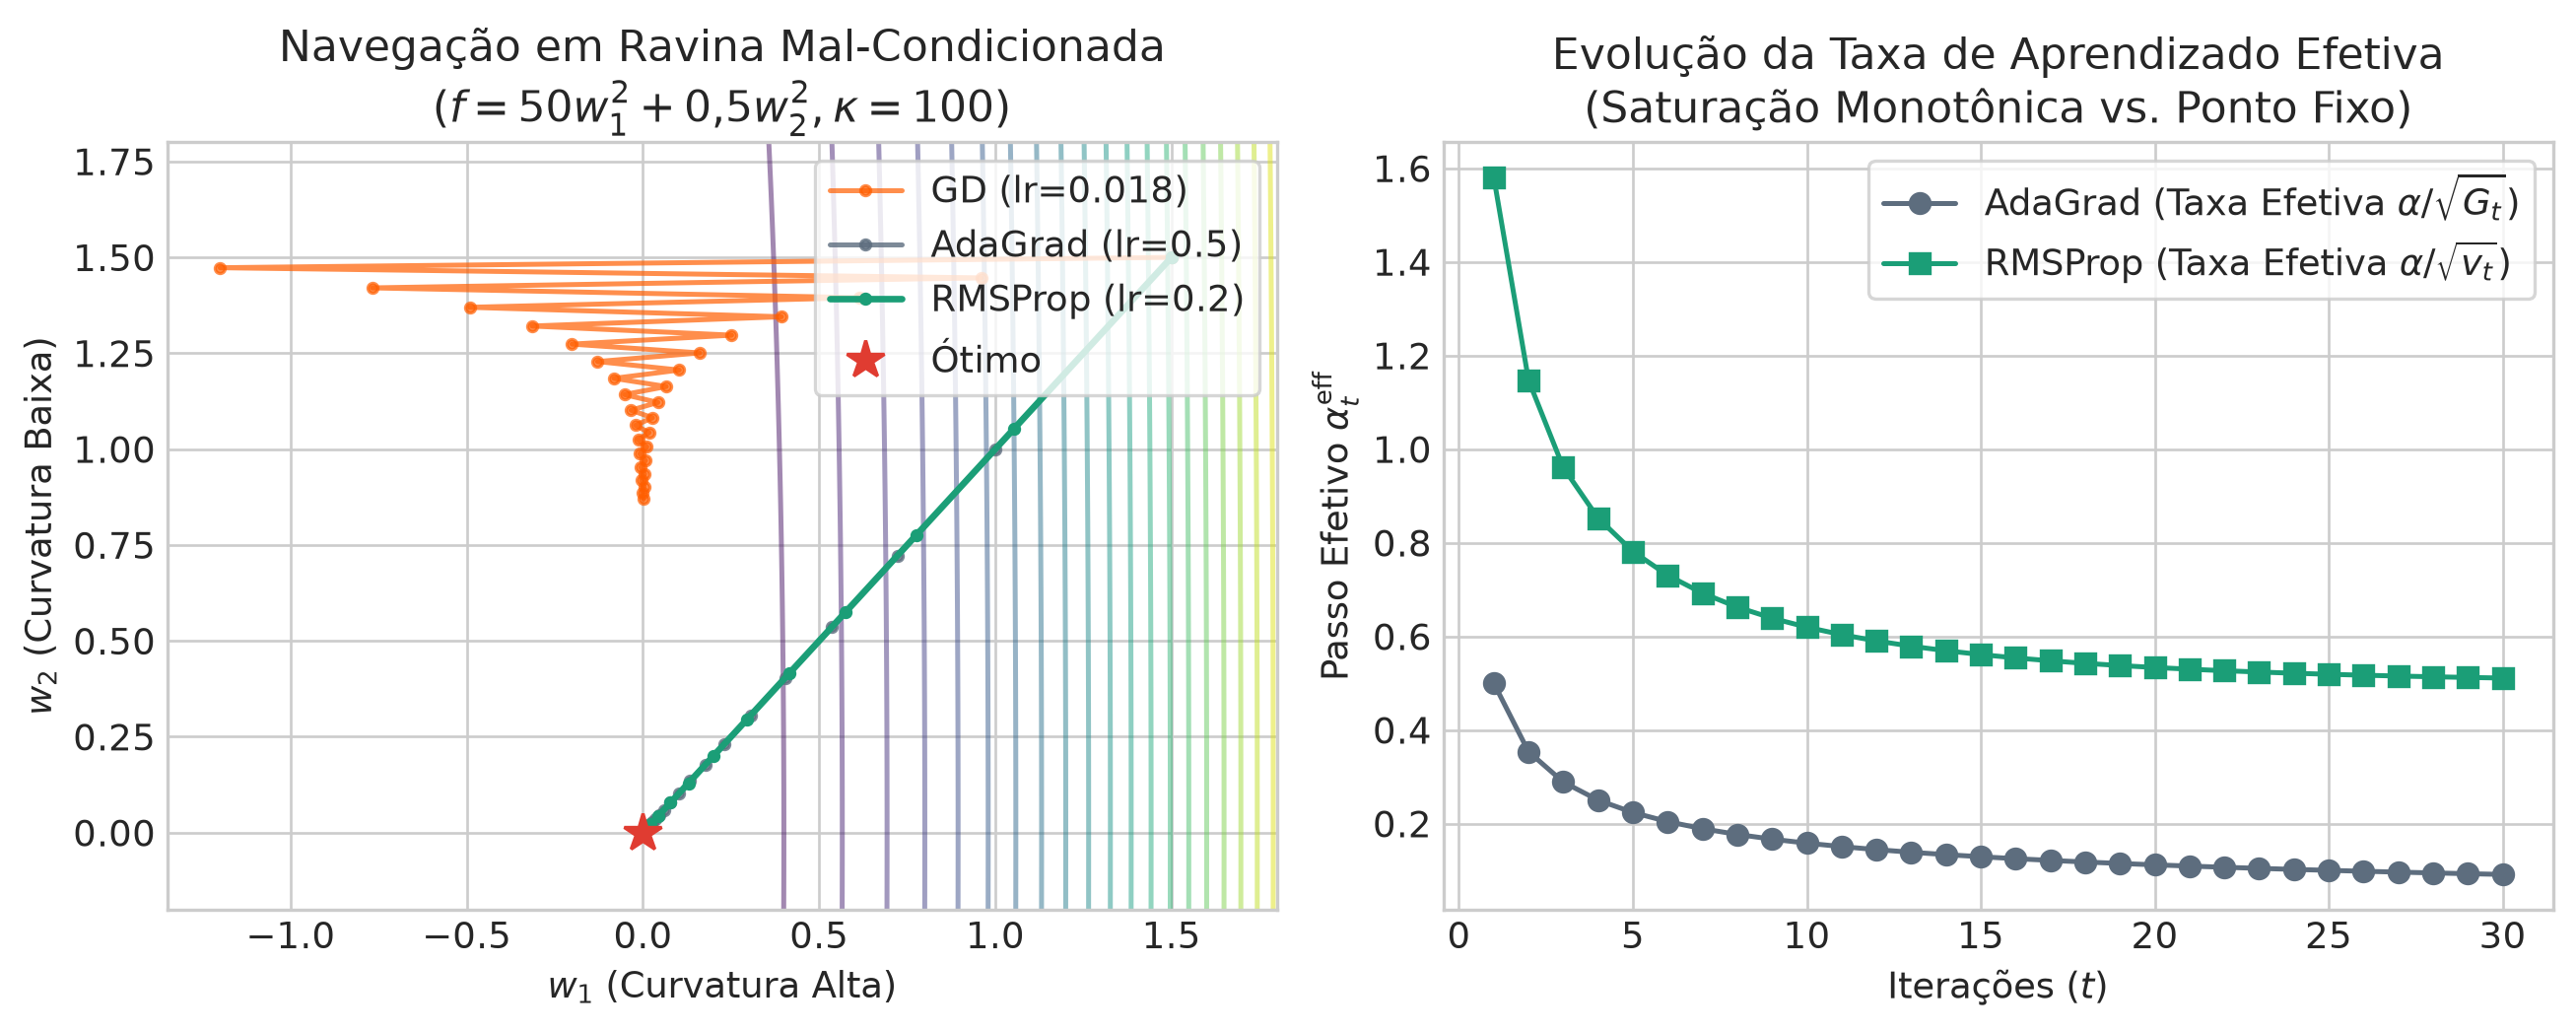
\includegraphics[width=0.88\textwidth]{figures/adagrad_vs_rmsprop.png}\\
  \vspace{0.2cm}
  {\footnotesize \textbf{À esquerda:} AdaGrad congela no meio da descida; RMSProp atinge o minimizador. \textbf{À direita:} Decaimento contínuo de $\alpha^{\text{eff}}$ no AdaGrad versus estabilização adaptativa no RMSProp.}
\end{frame}

% SLIDE 37: PAUSA 5
\begin{frame}{Pausa 5: AdaGrad vs. RMSProp}
  \begin{callouttip}[O Dilema da Memória]
    Por que o AdaGrad é considerado ideal para modelos com dados esparsos (como processamento de linguagem natural com vocabulários gigantescos), mas falha catastroficamente ao treinar redes neurais profundas de visão computacional com muitas épocas? Como o RMSProp resolve esse dilema?
  \end{callouttip}

  \begin{callouttip}[Propriedades dos Otimizadores Adaptativos]
    \begin{itemize}
      \item[\qmark] No AdaGrad, a sequência de acumuladores $G_{t, i}$ é monotonicamente não-decrescente.
      \item[\qmark] Em problemas com número infinito de passos, a taxa de aprendizado efetiva do AdaGrad converge para zero se os gradientes não se anularem.
      \item[\qmark] A constante $\beta_2 = 0{,}9$ no RMSProp implica que o otimizador descarta gradientes mais antigos que aproximadamente 10 iterações.
      \item[\qmark] O RMSProp utiliza segundas derivadas para calcular o vetor $\mathbf{v}_t$.
    \end{itemize}
  \end{callouttip}
\end{frame}

% SLIDE 38: PAUSA 5 - RESPOSTA
\begin{frame}{Pausa 5: AdaGrad vs. RMSProp --- Resposta}
  \begin{callouttip}[Propriedades dos Otimizadores Adaptativos --- Resposta]
    \begin{itemize}
      \item[\cmark] \textbf{Verdadeiro.} Como $g^2 \ge 0$, a soma acumulada de quadrados nunca diminui ($G_t \ge G_{t-1}$).
      \item[\cmark] \textbf{Verdadeiro.} Para séries de gradientes não nulos, o denominador cresce indefinidamente e a taxa efetiva colapsa para zero.
      \item[\cmark] \textbf{Verdadeiro.} Trata-se da meia-vida de decaimento geométrico $\sum k \beta_2^k (1-\beta_2) \approx \frac{1}{1-\beta_2}$.
      \item[\xmark] \textbf{Falso.} O RMSProp é puramente de primeira ordem; utiliza apenas gradientes estocásticos obtidos via autodiff.
    \end{itemize}
  \end{callouttip}
  \vspace{0.2cm}
  \textbf{Voltando à pergunta:} Em textos, palavras raras aparecem pouco e mantêm $G_{t, i}$ pequeno, permitindo passos grandes quando finalmente ocorrem. Em redes profundas de visão, contudo, o treinamento dura centenas de milhares de passos; $G_t$ cresce tanto que o modelo congela precocemente. O RMSProp utiliza a EMA para ``esquecer'' o passado remoto, mantendo a taxa ativa perenemente.
\end{frame}

% ==============================================================================
% SEÇÃO: FECHAMENTO
% ==============================================================================
\begin{frame}[plain]
  \centering
  \vspace{2cm}
  {\Huge \textcolor{unicampblue}{\textbf{Fechamento}}}\\
  \vspace{0.5cm}
  {\large \textcolor{unicampteal}{Síntese e Ponte para a Aula 12}}
\end{frame}

% SLIDE 40
\begin{frame}{Retomando as 4 Perguntas}
  \begin{enumerate}
    \item \textbf{Passo de Newton:} Minimizador exato da Série de Taylor quadrática ($\Delta\mathbf{w}_{\text{nt}} = -H^{-1}\mathbf{g}$). Invariante sob transformações afins, converge quadraticamente perto do ótimo.
    \vspace{0.2cm}
    \item \textbf{Patologias em ML:} Custo proibitivo $\mathcal{O}(d^3)$, memória $\mathcal{O}(d^2)$ e armadilha em pontos de sela onde $H$ possui autovalores negativos.
    \vspace{0.2cm}
    \item \textbf{Precondicionamento Diagonal:} Transforma o espaço métrico e desacopla as coordenadas, reduzindo a complexidade de inversão e armazenamento para $\mathcal{O}(d)$.
    \vspace{0.2cm}
    \item \textbf{AdaGrad e RMSProp:} Usam as primeiras derivadas passadas como estimador da curvatura. O AdaGrad congela por acúmulo infinito; o RMSProp resolve com Média Móvel Exponencial (EMA).
  \end{enumerate}
\end{frame}

% SLIDE 41: TABELA SÍNTESE
\begin{frame}{Síntese: Do Passo Escalar ao RMSProp}
  \centering
  \resizebox{\textwidth}{!}{%
  \begin{tabular}{lcccc}
    \toprule
    \textbf{Otimizador} & \textbf{Informação} & \textbf{Custo / Passo} & \textbf{Memória} & \textbf{Comportamento em $\kappa \gg 1$} \\
    \midrule
    \textbf{GD / SGD} & $\nabla f$ (1ª ordem) & $\mathcal{O}(d)$ & $\mathcal{O}(d)$ & Ziguezague severo sob taxa escalar única \\
    \addlinespace
    \textbf{Newton Puro} & $\nabla f$ e $\nabla^2 f$ (2ª ordem) & $\mathcal{O}(d^3)$ & $\mathcal{O}(d^2)$ & Ótimo em 1 passo, mas proibitivo em escala \\
    \addlinespace
    \textbf{AdaGrad} & Histórico $\sum g^2$ & $\mathcal{O}(d)$ & $\mathcal{O}(d)$ & Ótimo em esparsos; congela em redes profundas \\
    \addlinespace
    \textbf{RMSProp} & EMA $\beta_2 v + (1-\beta_2)g^2$ & $\mathcal{O}(d)$ & $\mathcal{O}(d)$ & Escalas adaptativas perenes por coordenada \\
    \bottomrule
  \end{tabular}%
  }
\end{frame}

% SLIDE 42: PONTE
\begin{frame}{Ponte para a Aula 12: Momento e o Otimizador Adam}
  \begin{columns}[T]
    \begin{column}{0.48\textwidth}
      \textbf{O Que Vimos Hoje (Aula 11):}
      \begin{itemize}
        \item Precondicionamento diagonal equaliza escalas:
        \[w_{i, k+1} = w_{i, k} - \frac{\alpha}{\sqrt{v_{t, i}} + \epsilon} g_{t, i}\]
        \item Resolve o descompasso de escalas ($\kappa \gg 1$).
        \item \textbf{Falta inércia direcional:} ainda oscila se o gradiente apontar transversalmente!
      \end{itemize}
    \end{column}
    \begin{column}{0.48\textwidth}
      \textbf{O Próximo Passo (Aula 12):}
      \begin{itemize}
        \item Adicionar \textbf{massa física e momento}:
        \[m_t = \beta_1 m_{t-1} + (1 - \beta_1) g_t\]
        \item Momento de Polyak e Aceleração de Nesterov.
        \item \textbf{A Grande Síntese:} Unir $m_t$ (1º momento) com $v_t$ (2º momento) $\implies$ \textbf{Otimizador Adam e AdamW}!
      \end{itemize}
    \end{column}
  \end{columns}
\end{frame}

\end{document}
